\documentclass[border=5pt]{standalone}
\usepackage{pgfplots}
\pgfplotsset{compat=1.18}
\usepackage{siunitx}
\usepackage{tikz}
\usetikzlibrary{calc}

\definecolor{lr1}{RGB}{31,119,180}
\definecolor{lr2}{RGB}{255,127,14}
\definecolor{lr3}{RGB}{143,0,255}

\begin{document}
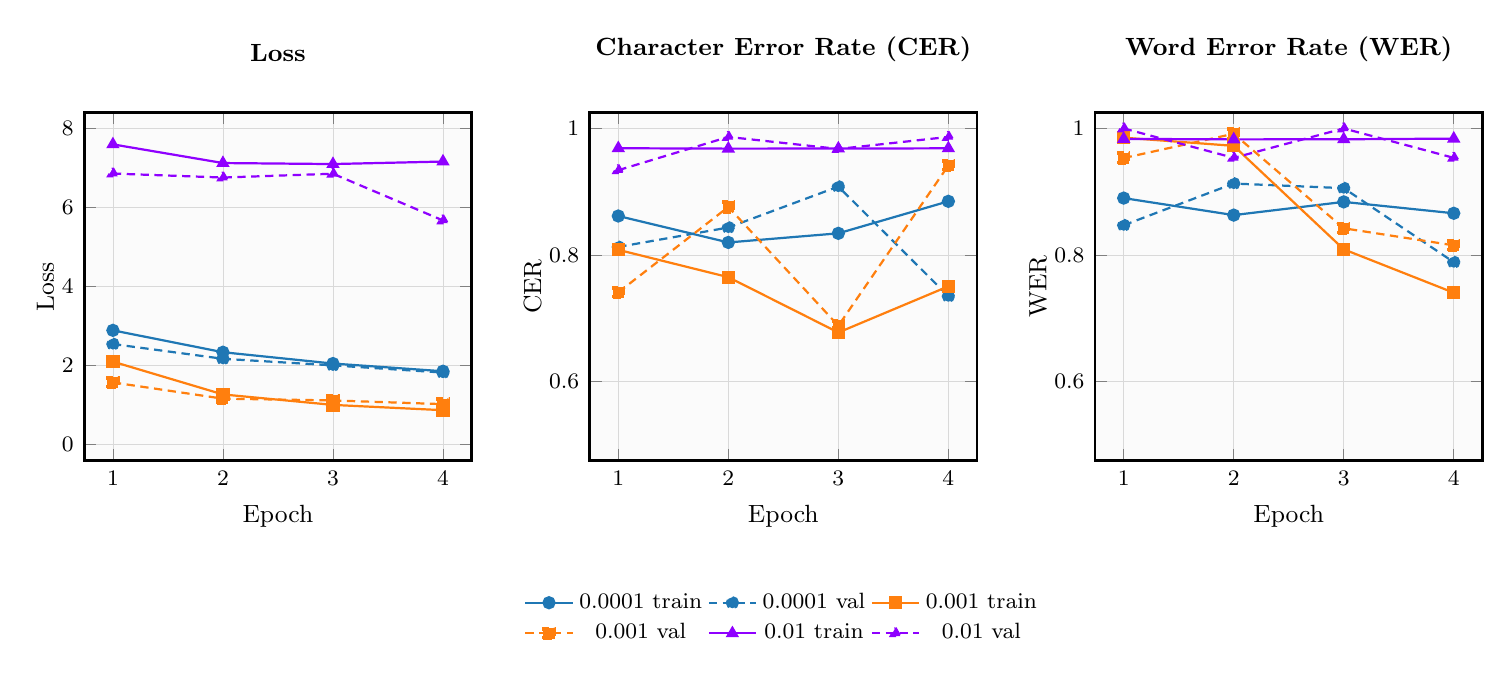
\begin{tikzpicture}[remember picture]

    % Графік 1: Loss
    \begin{axis}[
        name=plot1,
        width=6.5cm,
        height=6cm,
        xlabel={Epoch},
        ylabel={Loss},
        ylabel style={yshift=-0.15cm},
        xmin=0.9, xmax=4.1,
        ymin=0, ymax=8,
        xtick={1,2,3,4},
        grid=both,
        grid style={line width=.1pt, draw=gray!10},
        major grid style={line width=.2pt,draw=gray!30},
        title={Loss},
        axis background/.style={fill=gray!3},
        title style={yshift=3mm, font=\small\bfseries},
        label style={font=\small},
        tick label style={font=\footnotesize},
        line width=1pt,
        enlarge x limits=0.05,
        enlarge y limits=0.05,
        every axis plot/.append style={mark size=2pt},
        legend to name=commonlegend,
        legend columns=3,
        legend style={draw=none, fill=none, font=\footnotesize}
    ]
        % 0.0001
        \addplot[color=lr1, mark=*, thick] coordinates {(1,2.8933) (2,2.3398) (3,2.0535) (4,1.8585)};
        \addplot[color=lr1, mark=*, thick, densely dashed] coordinates {(1,2.5466) (2,2.1737) (3,2.0070) (4,1.8252)};

        % 0.001
        \addplot[color=lr2, mark=square*, thick] coordinates {(1,2.1017) (2,1.2720) (3,1.0073) (4,0.8735)};
        \addplot[color=lr2, mark=square*, thick, densely dashed] coordinates {(1,1.5756) (2,1.1651) (3,1.1202) (4,1.0268)};

        % 0.01
        \addplot[color=lr3, mark=triangle*, thick] coordinates {(1,7.5975) (2,7.1251) (3,7.0998) (4,7.1627)};
        \addplot[color=lr3, mark=triangle*, thick, densely dashed] coordinates {(1,6.8595) (2,6.7583) (3,6.8547) (4,5.6728)};

        \legend{0.0001 train, 0.0001 val, 0.001 train, 0.001 val, 0.01 train, 0.01 val}
    \end{axis}

    % Графік 2: CER, розташовується праворуч від plot1
    \begin{axis}[
        name=plot2,
        at={($(plot1.east)+(1.5cm,0)$)},
        anchor=west,
        width=6.5cm,
        height=6cm,
        xlabel={Epoch},
        ylabel={CER},
        ylabel style={yshift=-0.15cm},
        xmin=0.9, xmax=4.1,
        ymin=0.5, ymax=1.0,
        xtick={1,2,3,4},
        grid=both,
        grid style={line width=.1pt, draw=gray!10},
        major grid style={line width=.2pt,draw=gray!30},
        title={Character Error Rate (CER)},
        axis background/.style={fill=gray!3},
        title style={yshift=3mm, font=\small\bfseries},
        label style={font=\small},
        tick label style={font=\footnotesize},
        line width=1pt,
        enlarge x limits=0.05,
        enlarge y limits=0.05,
        every axis plot/.append style={mark size=2pt}
    ]
        % 0.0001
        \addplot[color=lr1, mark=*, thick] coordinates {(1,0.8616) (2,0.8198) (3,0.8342) (4,0.8848)};
        \addplot[color=lr1, mark=*, thick, densely dashed] coordinates {(1,0.8127) (2,0.8434) (3,0.9081) (4,0.7348)};

        % 0.001
        \addplot[color=lr2, mark=square*, thick] coordinates {(1,0.8081) (2,0.7649) (3,0.6774) (4,0.7504)};
        \addplot[color=lr2, mark=square*, thick, densely dashed] coordinates {(1,0.7409) (2,0.8759) (3,0.6881) (4,0.9415)};

        % 0.01
        \addplot[color=lr3, mark=triangle*, thick] coordinates {(1,0.9687) (2,0.9681) (3,0.9682) (4,0.9686)};
        \addplot[color=lr3, mark=triangle*, thick, densely dashed] coordinates {(1,0.9340) (2,0.9866) (3,0.9676) (4,0.9866)};
    \end{axis}

    % Графік 3: WER, розташовується праворуч від plot2
    \begin{axis}[
        name=plot3,
        at={($(plot2.east)+(1.5cm,0)$)},
        anchor=west,
        width=6.5cm,
        height=6cm,
        xlabel={Epoch},
        ylabel={WER},
        ylabel style={yshift=-0.15cm},
        xmin=0.9, xmax=4.1,
        ymin=0.5, ymax=1.0,
        xtick={1,2,3,4},
        grid=both,
        grid style={line width=.1pt, draw=gray!10},
        major grid style={line width=.2pt,draw=gray!30},
        title={Word Error Rate (WER)},
        axis background/.style={fill=gray!3},
        title style={yshift=3mm, font=\small\bfseries},
        label style={font=\small},
        tick label style={font=\footnotesize},
        line width=1pt,
        enlarge x limits=0.05,
        enlarge y limits=0.05,
        every axis plot/.append style={mark size=2pt}
    ]
        % 0.0001
        \addplot[color=lr1, mark=*, thick] coordinates {(1,0.8899) (2,0.8630) (3,0.8839) (4,0.8659)};
        \addplot[color=lr1, mark=*, thick, densely dashed] coordinates {(1,0.8470) (2,0.9129) (3,0.9056) (4,0.7886)};

        % 0.001
        \addplot[color=lr2, mark=square*, thick] coordinates {(1,0.9854) (2,0.9725) (3,0.8089) (4,0.7403)};
        \addplot[color=lr2, mark=square*, thick, densely dashed] coordinates {(1,0.9532) (2,0.9916) (3,0.8422) (4,0.8152)};

        % 0.01
        \addplot[color=lr3, mark=triangle*, thick] coordinates {(1,0.9835) (2,0.9827) (3,0.9829) (4,0.9839)};
        \addplot[color=lr3, mark=triangle*, thick, densely dashed] coordinates {(1,1.0) (2,0.9535) (3,1.0) (4,0.9535)};
    \end{axis}

    % Розміщення загальної легенди під усіма графіками
    \node at ($(plot1.south)!0.5!(plot3.south)+(0,-2.0cm)$) {\pgfplotslegendfromname{commonlegend}};
    
\end{tikzpicture}
\end{document}